\documentclass[letterpaper, 12pt]{math}

\usepackage{amsmath}
\usepackage{amssymb}
\usepackage{pgfplots}
\pgfplotsset{
  integral axis/.style={
    axis lines=middle,
    enlarge y limits=upper,
    axis equal image, width=12cm,
    xlabel=$x$, ylabel=$y$,
    ytick=\empty,
    xticklabel style={font=\small, text height=1.5ex, anchor=north},
    samples=100
  },
  integral/.style={
    domain=2:10,
    samples=9
  },
  integral fill/.style={
    integral,
    draw=none, fill=#1,
  },
  integral fill/.default=cyan!10,
  integral line/.style={
    integral,
    very thick,
    draw=#1
  },
  integral line/.default=black
}

\title{Approximate Integration}
\author{Alvin Lin}
\date{Calculus II: August 2016 - December 2016}

\begin{document}

\maketitle

\section*{Approximate Integration}
\[ \int_{0}^{1}{\e^{x^{2}}\diff{x}} \]
Normally we would solve this problem by integrating
\( \int{\e^{x^{2}}} = F(x) \) and
then using the Fundamental Theorem of Calculus (\( F(1)-F(0) \)). However, there
is no known way to integrate \( \e^{x^{2}} \) (or at least it becomes very
difficult). We can find a numerical approximation of it instead.
\[ \int_{a}^{b}{f(x)\diff{x}} = \lim_{\Delta x \to 0}
   \sum_{i=1}^{n}{f(x_{i}^{*})\Delta x} \]
\[ x_{i}^{*}\in\bigg[x_{i-1},x_{i}\bigg] \]
\[ \Delta x = \frac{b-a}{n} \]
When we integrate, we are taking the sum of areas of rectangles under the curve
as the width of the rectangle approaches 0.This gives us an exact value. If we
cannot do that, then we can approximate the integral by removing the limit.
\[ \int_{a}^{b}{f(x)\diff{x}} \approx \sum_{i=1}^{n}{f(x_{i}^{*})\Delta x} \]
This splits the integral into \( n \) discrete points, each of which we can
calculate a rectangular area from.

\subsubsection*{Left Riemann Sum Approximation}
\[ L_{n} = \sum_{i=1}^{n}{f(x_{i-1})\Delta x} \]
\[ = \Delta x\bigg[f(x_{0})+f(x_{1})+...+f(x_{n-1})\bigg] \]
If we split the area under the curve into \(n\) sections, we can use
\( f(x_{i}) \) as the height of \textbf{the left side of a rectangle} under the
curve. By calculating the sum of the areas of the \(n\) rectangles starting from
\( x_{0} \), we achieve the left Riemann sum approximation of the integral.
\begin{center}
  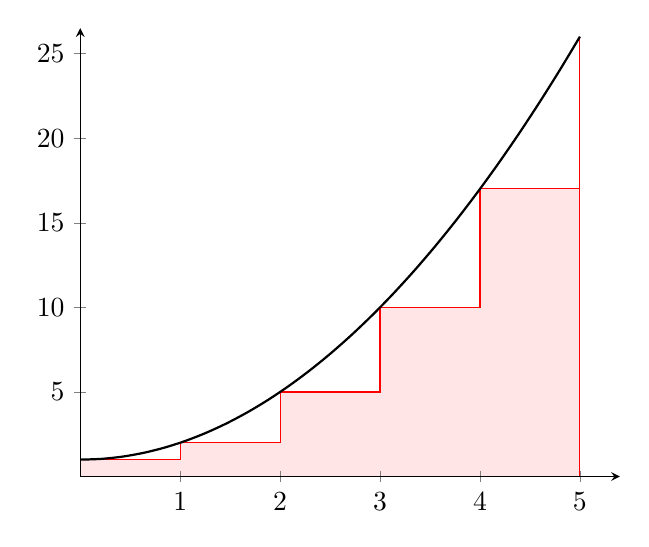
\begin{tikzpicture}
    \begin{axis}[
      xtick={0,...,5},ytick={5,10,15,20,25},
      xmax=5.4,ymax=26.5,ymin=0,xmin=0,
      enlargelimits=true,
      axis lines=middle,
      clip=false,
      domain=0:5,
      axis on top
    ]
    \addplot [draw=red, fill=red!10, const plot mark left, samples=6]
      {1+x^2} \closedcycle;
    \addplot[smooth, thick,domain=0:5]{1+x^2};
    \end{axis}
  \end{tikzpicture}
\end{center}

\subsubsection*{Right Riemann Sum Approximation}
\[ R_{n} = \sum_{i=1}^{n}{(f(x_{i})\Delta x} \]
\[ = \Delta x\bigg[f(x_{1})+f(x_{2})+...+f(x_{n})\bigg] \]
If we split the area under the curve into \(n\) sections, we can use
\( f(x_{i}) \) as the height of \textbf{the right side of a rectangle} under the
curve. By calculating the sum of the areas of the \(n\) rectangles starting from
\( x_{1} \), we achieve the right Riemann sum approximation of the integral.
\begin{center}
  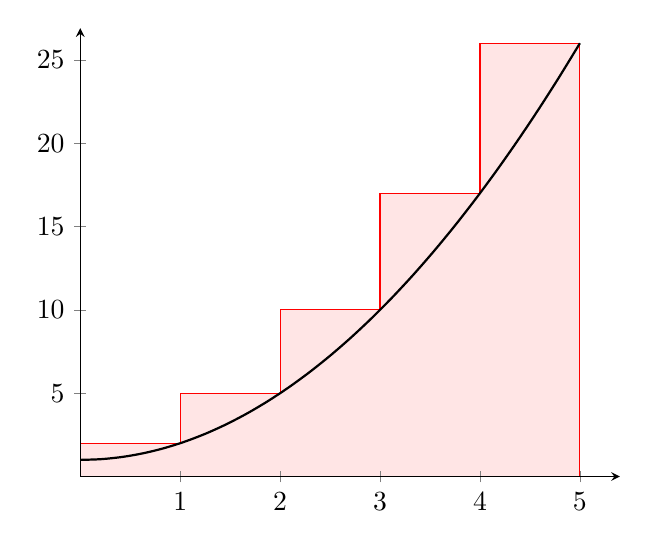
\begin{tikzpicture}
    \begin{axis}[
      xtick={0,...,5}, ytick={5,10,15,20,25},
      xmax=5.4, ymax=26.9, ymin=0, xmin=0,
      enlargelimits=true,
      axis lines=middle,
      domain=0:5,
      axis on top
    ]
    \addplot [draw=red, fill=red!10, const plot mark right, samples=6]
      {1+x^2} \closedcycle;
    \addplot[smooth, thick,domain=0:5]{1+x^2};
    \end{axis}
  \end{tikzpicture}
\end{center}

\subsubsection*{Midpoint Approximation}
\[ M_{n} = \sum_{i=1}^{n}{f(\bar{x}_{i})\Delta x} \]
\[ = \Delta x\bigg[f(\bar{x}_{i})+f(\bar{x}_{2})+...+f(\bar{x}_{n})\bigg] \]
\[ \mathrm{where} \quad \bar{x}_{i} = \frac{x_{i-1}+x_{i}}{2} \]
If we split the area under the curve into \( n \) sections, we can calculate the
midpoints between each section \( \bar{x}_{i} \). We can use
\( f(\bar{x}_{i}) \) as the heights of our rectangles and by summing up the
areas of the rectangles, we achieve the midpoint approximation of the integral.
\begin{center}
  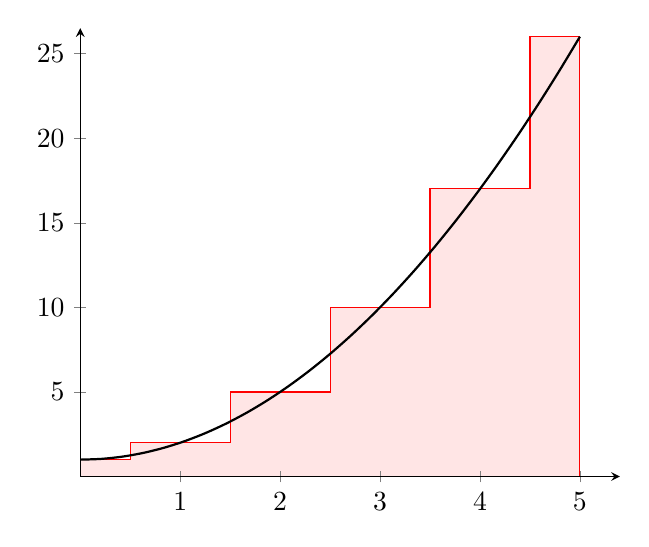
\begin{tikzpicture}
    \begin{axis}[
      xtick={0,...,5},ytick={5,10,15,20,25},
      xmax=5.4,ymax=26.5,ymin=0,xmin=0,
      enlargelimits=true,
      axis lines=middle,
      clip=false,
      domain=0:5,
      axis on top
    ]
    \addplot [draw=red, fill=red!10, const plot mark mid, samples=6]
      {1+x^2} \closedcycle;
    \addplot[smooth, thick,domain=0:5]{1+x^2};
    \end{axis}
  \end{tikzpicture}
\end{center}

\subsubsection*{Trapezoidal Rule Approximation}
\[ T_{n} = \frac{\Delta x}{2}
   \bigg[f(x_{0})+2f(x_{1})+...+2f(x_{n-1})+f(x_{n})\bigg] \]
If we split the area under the curve into \( n \) sections, we can use
\( f(x_{i}) \) as bases of trapezoids. By summing up the areas of the
trapezoids, we achieve the trapezoidal approximation of the integral.
\begin{center}
  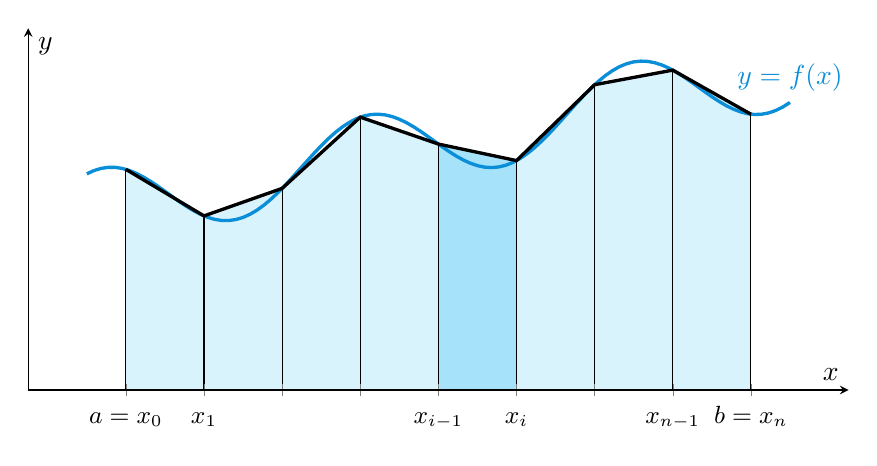
\begin{tikzpicture}[
    declare function={f=x/5-cos(deg(x*1.85))/2+2;}
  ]
    \begin{axis}[
      integral axis,
      ymin=0,
      xmin=0.75, xmax=11.25,
      domain=1.5:10.5,
      xtick={2,...,10},
      xticklabels={$a=x_0$, $x_1$,,,$x_{i-1}$,$x_i$,,$x_{n-1}$,$b=x_n$},
      axis on top
    ]
      \addplot [integral fill=cyan!15] {f} \closedcycle;
      \addplot [integral fill=cyan!35, domain=6:7, samples=2] {f} \closedcycle;
      \addplot [very thick, cyan!75!blue] {f} node [anchor=south] {$y=f(x)$};
      \addplot [integral line=black] {f};
      \addplot [integral, ycomb] {f};
    \end{axis}
  \end{tikzpicture}
\end{center}

\subsubsection*{Simpson's Rule}
\[ S_{n} = \frac{\Delta x}{3}
   \bigg[f(x_{1})+4f(x_{1})+2f(x_{2})+...+
   2f(x_{n-2})+4f(x_{n-1})+f(x_{n})\bigg] \]
Simpson's rule tries to get a parabolic approximation of the integral at every
\( n^{th} \) segment.
\begin{center}
  No visualization
\end{center}

\section*{Example}
\[ \int_{0}^{2}{\frac{x}{1+x^{2}}\diff{x}} =
   \bigg[\frac{1}{2}\ln|1+x^{2}|\bigg]_{0}^{2} \]
\[ = \frac{1}{2}\ln(5)-0 \]
\[ \approx 0.804719 \]
If we use the left Riemann sum approximation with n = 10:
\[ L_{n} = \Delta x\bigg[f(x_{i})+f(x_{2})+...+f(x_{n})\bigg] \]
\[ \Delta x = \frac{2-0}{10} \]
\[ = \frac{2}{10}\bigg[f(0)+f(\frac{2}{10})+...+f(\frac{18}{10})\bigg] \]
\[ \approx 0.708985... \]
If we use the right Riemann sum approximation with n = 10:
\[ R_{n} = \Delta x\bigg[f(x_{1})+f(x_{2})+...+f(x_{n})\bigg] \]
\[ \Delta x = \frac{2-0}{10} \]
\[ = \frac{2}{10}\bigg[f(\frac{2}{10})+f(\frac{4}{10})+...+f(2)\bigg] \]
\[ \approx 0.798391... \]
If we use the midpoint sum approximation with n = 10:
\[ M_{n} = \Delta x\bigg[
   f(\bar{x}_{i})+f(\bar{x}_{2})+...+f(\bar{x}_{n})\bigg] \]
\[ \Delta x = \frac{2-0}{10} \]
\[ = \frac{2}{10}\bigg[
   f(\frac{1}{10})+f(\frac{3}{10})+...+f(\frac{19}{20})\bigg] \]
\[ \approx 0.715920... \]
If we use the trapezoidal rule approximation with n = 10:
\[ T_{n} = \frac{\Delta x}{2}\bigg[
   f(x_{0})+2f(x_{1})+...+2f(x_{n-1})+f(x_{n})\bigg] \]
\[ \Delta x = \frac{2-0}{10} \]
\[ = \frac{2}{10}\times\frac{1}{2}\bigg[
   f(0)+2f(\frac{2}{10})+...+2f(\frac{18}{20})+f(2)\bigg] \]
\[ \approx 0.753688 \]
If we use Simpson's Rule with n = 10:
\[ S_{n} = \frac{\Delta x}{3}\bigg[
   f(x_{1})+4f(x_{1})+2f(x_{2})+...+2f(x_{n-2})+4f(x_{n-1})+f(x_{n})\bigg] \]
\[ \Delta x = \frac{2-0}{10} \]
\[ = \frac{2}{10}\times\frac{1}{3}\bigg[
   f(0)+4f(\frac{2}{10})+2f(\frac{4}{10})...+4f(\frac{18}{20})+f(2)\bigg] \]
\[ \approx 0.716586 \]

\begin{center}
  If any errors are found, please contact me at alvin.lin.dev@gmail.com
\end{center}

\end{document}
